% ---------------------------------------------------------------------
\documentclass{article}

% \usepackage{nberpreamble}
\usepackage{color}
\usepackage[dvipsnames]{xcolor}
\usepackage{fontspec}
\fontspec{Open Sans}
\setmainfont{Open Sans Light}
\usepackage{pgfplots}
\usepackage{tikz}
\usetikzlibrary{
  arrows,
  patterns,
  positioning,
  calc,
  fit,
  intersections,
  decorations.text,
  decorations.markings,
  decorations.pathmorphing,
  shadows.blur
}

\pgfplotsset{
  compat      = newest,
  axis x line = middle,
  axis y line = center,
  tick align  = outside,
  yticklabels = {,,},
  xticklabels = {,,},
  xtick       = {0},
  ytick       = {0}
}

% ---------------------------------------------------------------------
\begin{document}

\newcommand\cola{fill=red!20}
\newcommand\colb{fill=blue!20}
\begin{figure}
  \centering
  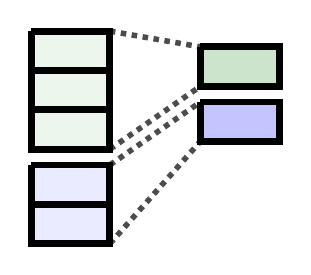
\begin{tikzpicture}[scale=1]
  % Group data
  \draw [line width = 2.5pt, fill=ForestGreen!8] ( 0.0,  1.0) -- (1.0,  1.0) -- (1.0,  0.5) -- ( 0.0,  0.5) -- ( 0.0,  1.0);
  \draw [line width = 2.5pt, fill=ForestGreen!8] ( 0.0,  0.5) -- (1.0,  0.5) -- (1.0,  0.0) -- ( 0.0,  0.0) -- ( 0.0,  0.5);
  \draw [line width = 2.5pt, fill=ForestGreen!8] ( 0.0,  0.0) -- (1.0,  0.0) -- (1.0, -0.5) -- ( 0.0, -0.5) -- ( 0.0,  0.0);

  \draw [line width = 2.5pt, fill=blue!8] ( 0.0, -0.7) -- (1.0, -0.7) -- (1.0, -1.2) -- ( 0.0, -1.2) -- ( 0.0, -0.7);
  \draw [line width = 2.5pt, fill=blue!8] ( 0.0, -1.2) -- (1.0, -1.2) -- (1.0, -1.7) -- ( 0.0, -1.7) -- ( 0.0, -1.2);

  % Collapsed data
  \draw [line width = 2.5pt, fill=ForestGreen!23] ( 2.15,  0.8) -- (3.15,  0.8) -- (3.15,  0.3) -- ( 2.15,  0.3) -- ( 2.15,  0.8);
  \draw [line width = 2.5pt, fill=blue!23]        ( 2.15,  0.1) -- (3.15,  0.1) -- (3.15, -0.4) -- ( 2.15, -0.4) -- ( 2.15,  0.1);

  % Link the two datasets
  \draw [line width = 2.0pt, opacity=0.7, dotted] (1.0,  1.0) -- ( 2.15,  0.8);
  \draw [line width = 2.0pt, opacity=0.7, dotted] (1.0, -0.5) -- ( 2.15,  0.3);

  \draw [line width = 2.0pt, opacity=0.7, dotted] (1.0, -0.7) -- ( 2.15,  0.1);
  \draw [line width = 2.0pt, opacity=0.7, dotted] (1.0, -1.7) -- ( 2.15, -0.4);
  \end{tikzpicture}
\end{figure}

%----------------------------------------------------------------------
\end{document}

